\documentclass[conference]{IEEEtran}
\IEEEoverridecommandlockouts
% The preceding line is only needed to identify funding in the first footnote. If that is unneeded, please comment it out.
\usepackage{cite}
\usepackage{amsmath,amssymb,amsfonts}
\usepackage{algorithmic}
\usepackage{graphicx}
\usepackage{textcomp}
\usepackage{xcolor}
\usepackage{hyperref}
\usepackage{nohyperref}
\usepackage{amstex}
\usepackage{enumitem}
\usepackage{float}
\newcommand{\BibTeX}{\textrm{B \kern -.05em \textsc{i \kern -.025em b} \kern -.08em
T \kern -.1667em \lower .7ex \hbox{E} \kern -.125emX}}
\begin{document}

    \title{Knowledge Discovery and Data Mining \hspace{2cm} Finals Report}

    \author{
        \IEEEauthorblockN{1\textsuperscript{st} 522H0036 - Luong Canh Phong}
        \IEEEauthorblockA{
            \textit{Faculty of Information Technology} \\
            \textit{Ton Duc Thang University}\\
            Ho Chi Minh City, Vietnam \\
            522H0036@student.tdtu.edu.vn
        }
        \and
        \IEEEauthorblockN{2\textsuperscript{nd} 520H0341 - Nguyen Thai Bao}
        \IEEEauthorblockA{
            \textit{Faculty of Information Technology} \\
            \textit{Ton Duc Thang University}\\ \
            Ho Chi Minh City, Vietnam \\
            520H0341@student.tdtu.edu.vn
        }
        \and
        \IEEEauthorblockN{3\textsuperscript{rd} 522H0030 - Le Tan Huy}
        \IEEEauthorblockA{
            \textit{Faculty of Information Technology} \\
            \textit{Ton Duc Thang University}\\
            Ho Chi Minh City, Vietnam \\
            522H0030@student.tdtu.edu.vn
        }
        \and
        \IEEEauthorblockN{4\textsuperscript{th} 522H0008 - Dao Minh Phuc}
        \IEEEauthorblockA{
            \textit{Faculty of Information Technology} \\
            \textit{Ton Duc Thang University}\\
            Ho Chi Minh City, Vietnam \\
            522H0008@student.tdtu.edu.vn
        }
        \and
        \IEEEauthorblockN{5\textsuperscript{th} 522H0136 - Nguyen Nhat Phuong Anh}
        \IEEEauthorblockA{
            \textit{Faculty of Information Technology} \\
            \textit{Ton Duc Thang University}\\
            Ho Chi Minh City, Vietnam \\
            522H0136@student.tdtu.edu.vn
        }
    }

    \maketitle

    \begin{abstract}
        Spam emails are a common problem seen on the internet as it is an annoyance in daily life and a cyber security risks to any sensitive and important data of a person or an organization/business.
        With the number of spam emails increasing more and more significantly over the past few years, many more algorithms are created and improved in spam detection efficiency.
        Overall, this paper goes through the basic understanding of spam emails, understanding the necessity of a spam classification algorithm, and learn more about the methodologies, its effectiveness and usefulness when detecting spam emails.
    \end{abstract}


    \section{Introduction}
    \label{sec:introduction}
    Since the birth of the Internet, spam email has been a common occurrence.
    Along with the rapid growth and widespread of the Internet, the frequency has been increasing significantly, especially over the past decade.
    In addition to being nuisances, a waste of time and email storage, spam emails can be sent with malicious intent of stealing information, hijacking devices by storing malware within the content of the email itself.
    And with the nature of email spam being sent by botnets, it isn't easy to avoid the situation due to a new bot can be easily created in case another one got blocked or banned on the site.
    A common way how most platforms (such as Gmail, Yahoo!, Outlook) handle these spams is to develop a Machine Learning (ML) model to detect and get rid of the spam emails, lowering the number of spams getting into the inbox.


    \section{Importance of Spam Classification}
    \label{sec:importance-of-spam-classification}
    To understand why spam classification is important to our lives, we must first understand the spam emails and its impact on daily life and businesses.
\subsection{Different Types of Spam Emails}
\label{subsec:different-types-of-spam-emails}

There are various forms of spam, sent with different intentions and purposes.
But they're commonly grouped into:

\begin{itemize}
    \item Phishing Emails: (TBA)
    \item Email Spoofing: (TBA)
    \item Tech support scams: (TBA)
    \item Current event scams: (TBA)
    \item Marketing/advertising email: (TBA)
    \item Malware scam: (TBA)
\end{itemize}

\subsection{Problems with Spam Emails}
\label{subsec:problems-with-spam-emails}

According to statistics report in 2023, 160 billion spam emails are sent every day, which is 46\% of the 347 billion emails sent on a daily basis.
Out of which, the most common type being marketing/advertising emails, which take up around 36\%, followed up with promotional of adult content, around 31.7\% of total spam emails. Despite scam and fraudulent emails is the least common type, over 70\% of them are phishing emails which is still over 6 billion phishing emails are being sent to users daily.

A single spam email carbon emission is almost 0.03g of CO2e, with the amount of spam being sent daily, it can easily get nearly 5 tonnes of CO2e being released every day.
Additionally, two-thirds of spam receivers have been reported to have their mental health affected due to the number of spam or phishing scams.

For businesses, this spam can be sent as a way to get businesses to invest in nonexistent organizations under the disguise of an investment and promised the payback would be worth the money spent, for individuals it would be under the form of bitcoin investment or for a chartiable cause.
Once the money is received, the sender would delete all traces and block the recipient contact.

\section{Methodologies for Spam Classification}
\label{sec:methodologies-for-spam-classification}

Many methods to prevent spam are applied; a commonly used method is using Machine Learning models like Random Forest (RF), Support Vector Machine (SVM), Logistic Regression (LR), Naive Bayes (NB) or Deep Learning models such as Artificial Neural Network (ANN),
(Explantion of used algorithms)


    \section{Reading and Understanding the Dataset}
    \label{sec:reading-and-understanding-the-dataset}
    After defining the business goals and the goals of data mining in the Business Understanding phase, the next crucial step in the CRISP-DM process is Data Understanding.
This phase involves collecting the initial dataset, examining its structure, and verifying data quality.
The primary goal is to become familiar with the dataset, identify potential quality issues, and extract early insights.

\begin{figure}[H]
    \centering
    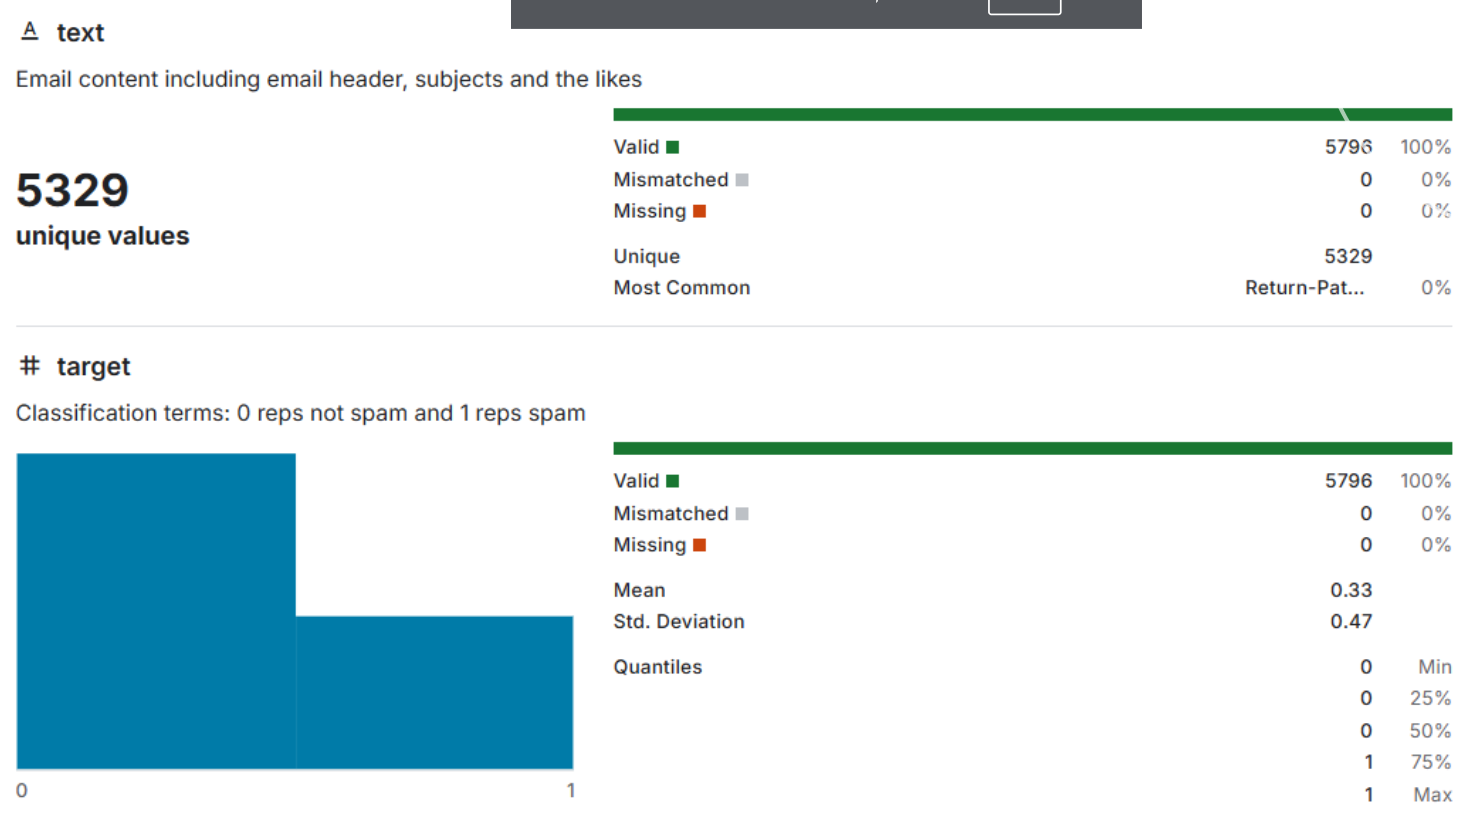
\includegraphics[width=\linewidth]{images/dataset_information}
    \caption{Dataset Information}
    \label{fig:dataset_information}
\end{figure}

In this image, we can see that out of all 5679 text values which included email headers, subjects and the likes, 5329 of them are unique values.
From this information, we can learn that the dataset has a large variety of values, and no duplicates are missing values that may impact the quality of the dataset significantly in any way.

Various NLP techniques were applied to explore the email content:

\subsection{Word Cloud}
\label{subsec:word-cloud}
Revealed high-frequency terms like number, url, date, mail, list, get, time, system, use, and HTML-related terms
(font, nbsp, td, tr).
The prevalence of number and url might indicate preprocessing/anonymization or simply be features of the emails.
HTML terms suggest formatted emails are common.

\begin{figure}[H]
    \centering
    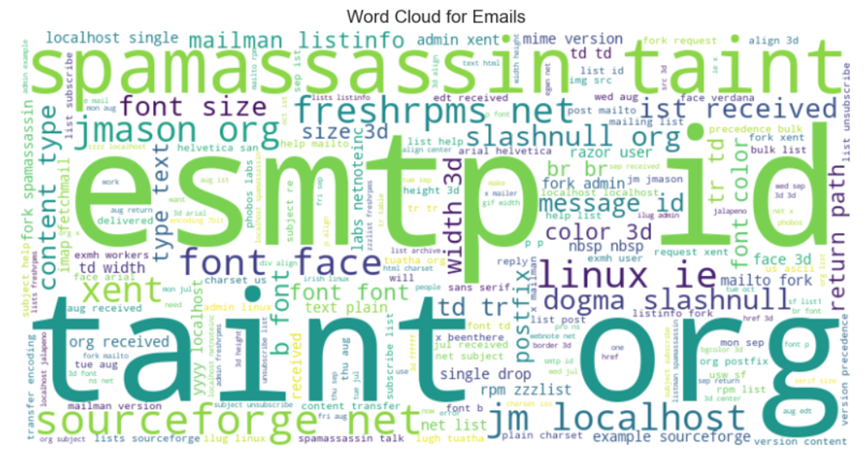
\includegraphics[width=\linewidth]{images/word_cloud}
    \caption{All emails in the form of Word Cloud}
    \label{fig:word_cloud}
\end{figure}

\smallskip
Prominent Keywords:

\begin{itemize}
    \item taint, spamassassin, esmtp, org, id, localhost, net, sourceforge: These are the largest and boldest words,indicating they are the most frequent and important terms within the analyzed email data.
    \item The rest of the word cloud: These words are smaller but still noticeable,suggesting they also play a significant role in the email context.
\end{itemize}

Possible Suggested Topics:

\begin{itemize}
    \item Spam Filtering: The presence of ``spamassassin'' and ``taint'' (often associated with marking suspicious emails) suggests a significant topic might be the identification and handling of spam.
    \item Mailing List Management: Words like ``list'',``listinfo'', ``mailman'', and ``mailing'' hint at discussions related to managing and interacting with email lists.
    \item Technical Email Information: Terms such as ``smtp'' (Simple Mail Transfer Protocol), ``mime'' (Multipurpose Internet Mail Extensions), ``version'',``id'', ``localhost'', and ``net'' indicate potential discussions about the technical aspects of email.
    \item Formatting and Display: Words like ``font'',``size'', ``face'', ``text'', and ``color'' might relate to how emails are displayed and formatted.
    \item Source and Path: ``sourceforge'' (an open-source software repository), ``received'', and ``path'' could be related to tracking the origin and route of emails.
    \item Related Systems and Software: ``linux'', ``xent'', and ``rpm'' might be the names of operating systems or software mentioned within the email context.
\end{itemize}

\subsection{Word Frequency (Top 10)}
\label{subsec:word-frequency}
After removing basic English stopwords and non-alphabetic tokens, the bar chart confirmed the dominance of words like number, url, mail, date, list, get.
Their persistence highlights their potential importance or noise factor.

\begin{figure}[H]
    \centering
    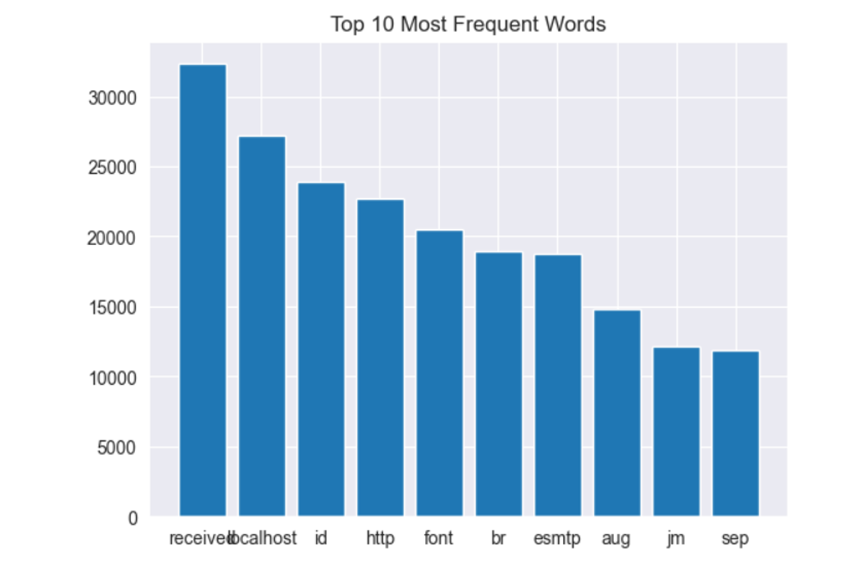
\includegraphics[width=\linewidth]{images/frequent_words}
    \caption{Bar Chart for 10 Most Frequent Words}
    \label{fig:frequent_words}
\end{figure}

The most frequent word is ``received'', with a significantly higher count (over 30,000) compared to the other top words.
This suggests that the word ``received'' appears very often in the analyzed text data after the filtering.

The following most frequent words, in descending order, are ``localhost'', ``id'', ``http'', ``font'', ``br'', ``esmtp'', ``aug'', ``jm'', and ``sep''.
These words have frequencies ranging from approximately 11,000 to 27,000.

The nature of the top words suggests the analyzed text data might be related to email headers or technical logs.
Words like ``received'', ``localhost'', ``id'', ``http'', and ``esmtp'' are commonly found in email metadata.
``aug'' and ``sep'' likely refer to month abbreviations.
``font'' and ``br'' could appear in the content or formatting information.

The code successfully identifies and counts the occurrences of words after applying basic text cleaning.
The use of nltk.word\_tokenize splits the text into individual words, .lower() converts them to lowercase for consistent counting, and the list comprehension filters out non-alphabetic tokens and common English stop words.

The Counter object efficiently calculates word frequencies, and most\_common(10) retrieves the top 10 most frequent words and their counts.
This data is then used to generate the bar chart using matplotlib.pyplot.

The visualization clearly shows the relative frequency of the top 10 words.
The height of each bar directly corresponds to the number of times that word appears in the processed text.


\subsection{Email Length Distribution}
\label{subsec:email-length-distribution}
The histogram showed a right-skewed distribution.
Most emails are short (under 500 words), but a long tail indicates the presence of very long outlier emails, adding diversity to the dataset structure.
Length could be a potential feature.

This code calculates how many words are in each email and then creates a bar chart (histogram) to show how many emails fall into different length categories (e.g., 0–500 words, 500–1000 words, etc.). It helps visualize the typical length of emails in our dataset.

\begin{figure}[H]
    \centering
    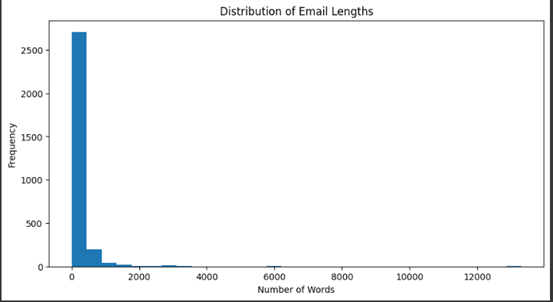
\includegraphics[width=\linewidth]{images/email_length_distribution}
    \caption{Bar Chart for Email Length Distribution}
    \label{fig:email_length_distribution}
\end{figure}

Distribution Shape:
\begin{itemize}
    \item Right-skewed: The majority of the bars are concentrated on the left side of the histogram, indicating that most emails are short in length.
    \item High Peak on the Left: The first bar (near zero words) has a significantly higher height than the other bars,showing a large number of very short emails.
    \item Long Tail to the Right: The bars gradually decrease towards the right, but there are still some emails with considerable length, extending to several thousand words.
\end{itemize}



\subsection{Common N-grams (Trigrams)}
\label{subsec:common-n-grams}
Analysis of the top 10 trigrams showed patterns like ``wed number aug'', ``number aug number'', ``date number number'', suggesting frequent date/number sequences or mailing list headers (list listinfo mail).
These patterns might help identify specific email types.

\begin{figure}[H]
    \centering
    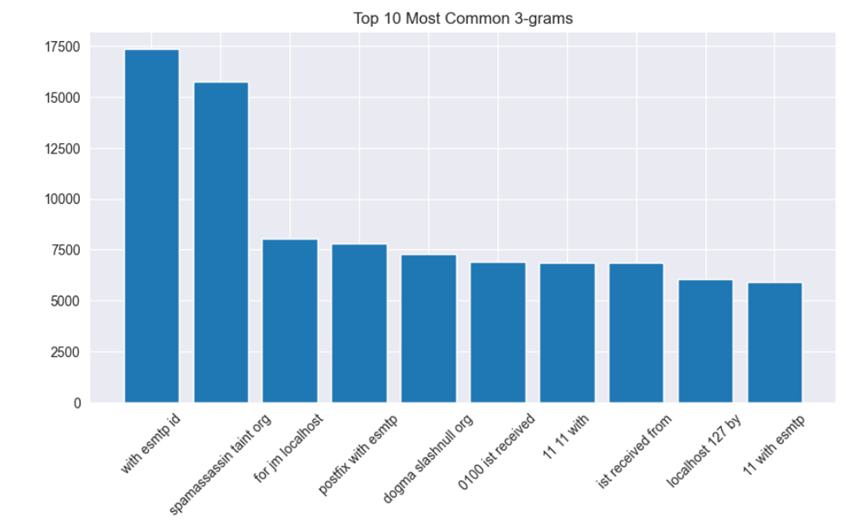
\includegraphics[width=\linewidth]{images/common_tri_grams}
    \caption{Bar Chart for 10 Most Common Trigrams}
    \label{fig:common_tri_grams}
\end{figure}

Observations:
\begin{itemize}
    \item The trigram ``with esmtp id'' is the most frequent, appearing significantly more often than the others.
    \item The trigram ``spamassassin taint org'' is the second most frequent.
    \item The remaining trigrams have lower and relatively similar frequencies.
    \item The trigrams suggest that the email data contains technical information, likely related to email headers and processing (``esmtp'', ``localhost'', ``received'') and spam filtering (``spamassassin'', ``taint'').
\end{itemize}

Potential Meaning:
\begin{itemize}
    \item The most frequent trigrams indicate the common occurrence of information related to email headers and the email transmission process.
    Phrases like ``with esmtp id'', ``postfix with esmtp'', ``ist received'', ``received from'', and ``localhost 127 by'' all pertain to how emails are sent and received.
    \item The presence of ``spamassassin taint org'' suggests that spam filtering activity is a significant aspect of this dataset.
    \item Other trigrams like ``for jm local/host'', ``dogma slashnull org'', ``0100 ist received'', ``11 11 with'', and ``11 with esmtp'' might relate to specific systems, software, or characteristic data formats within the context of this dataset.
\end{itemize}

Conclusion:

This chart reveals that information related to email processing and headers, as well as spam filtering activities, are prominent features in the analyzed text dataset.
The other trigrams may provide further insights into specific systems or formats relevant to this data.

\subsection{POS Tag Frequency}
\label{subsec:pos-tag-frequency}
The distribution of Part-of-Speech tags (NN, NNP, NNS, VB variants, JJ, IN being most frequent) confirmed that the email text follows typical English grammatical structures.

\begin{figure}[H]
    \centering
    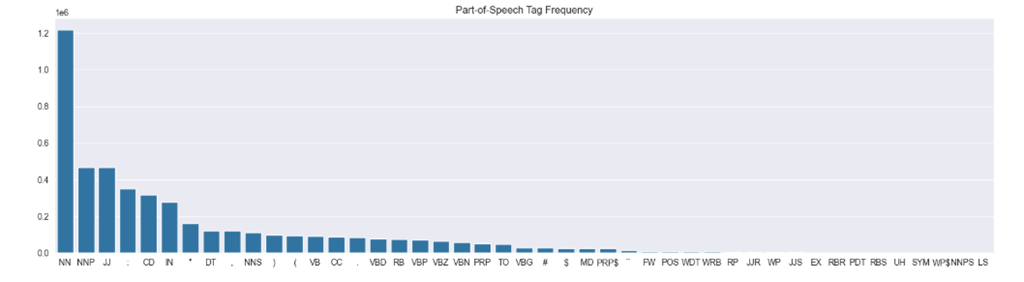
\includegraphics[width=\linewidth]{images/pos-tag-frequency}
    \caption{Bar Chart for POS Tag Frequency}
    \label{fig:pos-tag-frequency}
\end{figure}

Observations:
\begin{itemize}
    \item Nouns are highly frequent: The tags ``NN'' (singular nouns) and ``NNP'' (proper nouns) have the tallest bars,indicating they are the most frequent part-of-speech tags in this text.
    \item Adjectives and Prepositions/Conjunctions are also common: ``JJ'' (adjectives) and ``IN'' (prepositions/subordinating conjunctions) show relatively high frequencies as well.
    \item Verbs have varied frequencies: Different verb forms (``VB'', ``VBP'', ``VBZ'',``VBN'', ``VBG'') show varying levels of frequency, with the base form (``VB'') and non-3rd person singular present (``VBP'') being more common than others.
    \item Determiners are significant: ``DT'' (determiners like ``the'', ``a'', ``an'') also appear frequently.
    \item Other parts of speech are less frequent: Tags like adverbs (``RB''), pronouns (``PRP'', ``PRP\$''), modals (``MD''), coordinating conjunctions (``CC''), and various wh-words (``WDT'', ``WRB'', ``WP'', ``WP\$'') have noticeably lower frequencies compared to nouns and adjectives.
    \item Symbols and foreign words are rare: Tags like ``\$'' (dollar sign), ``FW'' (foreign word), and other symbols (``SYM'') have very short bars, indicating they are not common in this text.
\end{itemize}

\subsection{TF-IDF Visualization (Top 20)}
\label{subsec:tf-idf-visualization}
This analysis highlighted the importance of HTML tags and attributes (image, font, table, width, align, nbsp, size, color, etc.). These terms have high TF-IDF scores, indicating they are highly characteristic and useful for distinguishing between different emails, likely separating HTML-formatted emails from plain text ones.

TF-IDF combines two parts: Term Frequency (TF) and Inverse Document Frequency (IDF).

Term Frequency (TF): Measures how often a word appears in a document.
A higher frequency suggests greater importance.
If a term appears frequently in a document, it is likely relevant to the document’s content.
Formula:
\[
    \text{tf}(t, d) = \frac{f_{t,d}}{\sum_{t' \in d} f_{t',d}}
\]
where $f_{t,d}$ is the raw count of a term $t$ in a document, i.e., the number of times that term $t$ occurs in document $d$.
Note the denominator is simply the total number of terms in document $d$ (counting each occurrence of the same term separately).
There are various other ways to define term frequency:
\begin{itemize}
    \item The raw count itself: $\text{tf}(t,d) = f_{t,d}$
    \item Boolean ``frequencies'': $\text{tf}(t,d) = 1$ if $t$ occurs in $d$ and 0 otherwise;
    \item Logarithmically scaled frequency: $\text{tf}(t,d) = \log (1 + f_{t,d})$;
    \item Augmented frequency, to prevent a bias towards longer documents, e.g., raw frequency divided by the raw frequency of the most frequently occurring term in the document:
\end{itemize}
\[
    \text{tf}(t, d) = 0.5 + 0.5 \cdot \frac{f_{t,d}}{\max\{f_{t',d} : t' \in d\}}
\]

The inverse document frequency (IDF) is a measure of how much information the word provides, i.e., how common or rare it is across all documents.
It is the logarithmically scaled inverse fraction of the documents that contain the word (obtained by dividing the total number of documents by the number of documents containing the term, and then taking the logarithm of that quotient):
\[
    \text{idf}(t, D) = \log \frac{N}{|\{d : d \in D \text{ and } t \in d\}|}
\]

with
\begin{itemize}[leftmargin=2em, itemsep=0.5ex] % Adjust indentation as needed
    \item $N$: Total number of documents in the corpus $N = |D|$
    \item $|\{d \in D : t \in d\}|$: Number of documents where the term $t$ appears (e.g., $\text{tf}(t,d) \neq 0$). If the term is not in the corpus, this will lead to a division-by-zero.
    It is therefore common to adjust the numerator to $1+N$ and denominator to $1 + |\{d \in D : t \in d\}|$.
\end{itemize}

Term frequency--inverse document frequency (TF-IDF):
\[
    \text{tfidf}(t, d, D) = \text{tf}(t, d) \cdot \text{idf}(t, D)
\]

The TF-IDF scores highlight words that are important for distinguishing between different emails in your dataset.
While widespread words like ``the'' have high term frequency, their low inverse document frequency reduces their TF-IDF score because they appear in almost all emails.
Words with higher TF-IDF scores, like ``number' and ``url'' are likely more specific to certain subsets of your email data and could be valuable features for a classification task like spam detection.
The presence of ``you'' also suggests a potential distinction based on the direct address to the recipient.
This visualization helps identify terms that are characteristic of individual emails within the collection.

\begin{figure}[H]
    \centering
    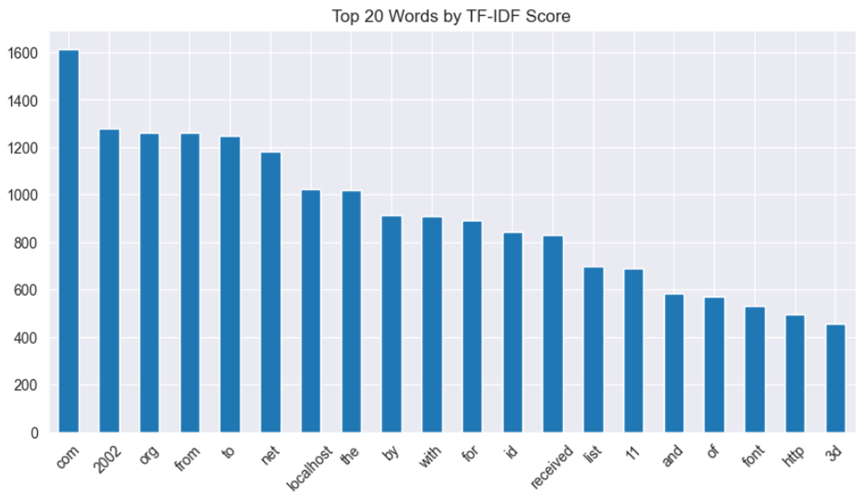
\includegraphics[width=\linewidth]{images/top_tf_idf_score}
    \caption{Bar Chart for Top 20 Words by TF-IDF Score}
    \label{fig:top_tf_idf_score}
\end{figure}

Observations:
\begin{itemize}
    \item ``com'' has the highest TF-IDF score: The word ``com'' has the tallest bar, indicating it has the highest TF-IDF score among the top 20.
    \item ``2002'' and ``org'' have the next highest scores: These words also have relatively high TF-IDF scores.
    \item Words like ``from'', ``to'', ``net'', and ``localhost'' have considerable scores: They suggest some importance in differentiating documents within the corpus.
    \item Common English words have lower scores: Words like ``the'', ``by'', ``with'', ``for'', ``and'', and ``of'' appear in the list but have lower TF-IDF scores compared to the more specific terms.
    This is expected because TF-IDF downweights words that appear frequently across many documents.
    \item Technical terms and identifiers are present: Words like ``id'', ``font'', ``http'', and ``3d'' suggest that these terms might be important in distinguishing certain types of documents within the corpus.
    \item ``received'' and ``list'' also have moderate TF-IDF scores.
    The number ``11'' also appears in the list.
\end{itemize}

Meaning of TF-IDF:
\begin{itemize}
    \item Term Frequency (TF): Measures how frequently a term appears in a document.
    \item Inverse Document Frequency (IDF): Measures how rare a term is across the entire corpus of documents.
    Words that appear in many documents have a lower IDF.
\end{itemize}

A high TF-IDF score for a word means that the word is frequent in a particular document but rare in the overall corpus.
Therefore, these words are considered more important for distinguishing documents.

In summary, this bar chart highlights the words that are most discriminative across the analyzed text documents based on their TF-IDF scores.
The words with higher scores, such as ``com'', ``2002'', ``org'', and ``localhost'', are likely good indicators of the specific content or categories of the documents in which they appear.
The presence of common English words with lower scores confirms the TF-IDF mechanism of prioritizing distinguishing terms.
This analysis is often used in information retrieval and text mining to identify the most relevant terms in a collection of documents.


    \section{Preprocessing the data}
    \label{sec:preprocessing-the-data}
    This section focuses on preparing the dataset for machine learning by cleaning and transforming the text data.
It includes removing unnecessary stop words, tokenizing the emails, and vectorizing the emails.

\subsection{Removing unnecessary stopwords}
\label{subsec:removing-unnecessary-stopwords}

\textbf{stop\_words = set(stopwords.words('english'))}: This line creates a set called stop\_words.
It uses the nltk library's stopwords module to get a list of common English words like ``the,'' ``a,'' ``is,'' etc., which are often removed from text data because they usually carry little meaningful information.
These words are converted into a set for efficient lookup during the removal process.

\textbf{puncture = set(string.punctuation)}: This line creates a set called puncture.
It uses the string library's punctuation attribute to get a list of punctuation marks.
Similar to stop\_words, these punctuation marks are converted into a set for efficient removal.

\textbf{def remove\_stopwords(text)}: This line defines a function named remove\_stopwords that takes a single argument, text, representing the input text to be processed.

\textbf{return ` '.join([word for word in text.split() if word not in stop\_words and word not in puncture])}: This line is the core of the function.
It uses a list comprehension to filter out stopwords and punctuation from the input text:

\begin{itemize}
    \item text.split(): This splits the input text into a list of individual words.
    \item if word not in stop\_words and word not in puncture: This condition checks if a word is not in either the stop\_words set or the puncture set.
    \item \text{[}word for \dots if \dots\text{]}: This creates a new list containing only the words that passed the condition.
    \item ` '.join(\ldots): This joins the words back together into a single string, separated by spaces.
\end{itemize}

Finally, the function returns this processed string (with stopwords and punctuation removed).
This step helps to reduce noise and focus on more meaningful words for further analysis.

\subsection{Tokenizing the emails}
\label{subsec:tokenizing-the-emails}

Each email was then tokenized, which involves splitting the text into individual words or tokens.

\textbf{import spacy}: This line imports the spacy library, a popular Python library for NLP tasks.

\textbf{nlp = spacy.load(`en\_core\_web\_sm')}: This line loads a specific language model within spaCy called en\_core\_web\_sm.
This model is trained on a large English text dataset and is used for various NLP operations, including schematization

\subsection{Defining and Applying the Lemmatization Function}
\label{subsec:defining-and-applying-the-lemmatization-function}

The next step involves reducing words to their base or root form, known as lemmatization, using the spaCy library.
This helps standardize words for better analysis.

\textbf{def lemmatize(email):}: This line defines a function named lemmatize that takes a single argument, ``email'', representing the input email text to be processed.

\textbf{doc = nlp(email)}: Inside the function, this line uses the previously loaded spaCy language model (``nlp'') to process the input ``email'' text.
The result, a spaCy Doc object containing tokens and their linguistic features, is stored in the ``doc'' variable.

\textbf{return ` '.join(token.lemma\_ for token in doc)}: This line performs the lemmatization and returns the result.
\begin{itemize}
    \item ``token.lemma\_ for token in doc'': This iterates through each token (word) in the processed ``doc'' object and extracts its lemma (base form).
    For example, ``running'' becomes ``run,'' ``studies'' become ``study.''
    \item `` ` '.join(\ldots)'': This joins the extracted lemmas back together into a single string, separated by spaces.
\end{itemize}
The function returns this lemmatized string.

\textbf{df['email'] = df['email'].apply(lemmatize)}: This line applies the ``lemmatize'' function to each entry in the ``email'' column of the pandas DataFrame named ``df''.
The original email text in the column is replaced by its lemmatized version.

This step is crucial for further analysis, as it allows the model to treat different forms of the same word (e.g., ``run,'' ``running,'' ``ran'') as a single concept, improving pattern recognition.

\subsection{Removing duplicate words}
\label{subsec:removing-duplicate-words}

This code snippet aims to remove duplicate words from each email string within the ``email'' column of the DataFrame ``df'', while importantly maintaining the original order of the remaining words.

\textbf{df[`email'] = \dots}: This part indicates that the result of the operation described on the right side will be assigned back to the ``email'' column of the ``df'' DataFrame, overwriting the previous content.

\textbf{df[`email'].apply(\dots)}: The ``apply()'' method is used here to apply a specific function to each element (each email string) in the ``email'' column.

\textbf{lambda x: \dots}: This defines an anonymous inline function (a lambda function).
The function takes one argument, ``x'', which represents an individual email string from the column during the ``apply'' operation.

\textbf{x.split()}: This part of the lambda function splits the input email string ``x'' into a list of individual words, using spaces as the default delimiter.

\textbf{set(x.split())}: This converts the list of words obtained from ``x.split()'' into a Python set.
A key property of sets is that they only store unique elements, so this step automatically removes any duplicate words present in the list.

\textbf{sorted(\dots, key=x.split().index)}: This is the core part for preserving order.
\begin{itemize}
    \item ``sorted(\ldots)'': This function sorts the elements of the set (which contains only unique words).
    \item ``key=x.split().index'': This is the crucial argument.
    It tells ``sorted'' not to sort alphabetically, but based on the index (position) of each unique word in the *original* list created by ``x.split()''.
    This effectively restores the initial sequence of words.
\end{itemize}

\textbf{` '.join(\dots)}: Finally, this joins the sorted (by original position), unique words back into a single string, with words separated by spaces.

Removing duplicate words can be beneficial in text processing tasks as it helps reduce redundancy and noise in the data, potentially leading to improved model performance.
Maintaining the original word order is important for preserving the contextual meaning of the email.

\subsection{Vectorizing}
\label{subsec:vectorizing}

To represent the processed email text numerically, a technique called vectorization was employed.
Specifically, TF-IDF (Term Frequency-Inverse Document Frequency) vectorization was used to convert the text into a numerical matrix that machine learning models can understand.
This step is crucial for training models to recognize patterns and make predictions based on email content.

\textbf{Creating the Vectorizer}

\textbf{TfidfVectorizer}: This line imports or initializes the ``TfidfVectorizer'' class from the ``sklearn.feature\_extraction.text'' library.
This class converts a collection of raw documents to a matrix of TF-IDF features.

\textbf{min\_df=1}: This parameter is set during the initialization of ``TfidfVectorizer''.
It specifies that a word must appear in at least one document (email, in this case) to be considered part of the vocabulary.
Setting it to 1 includes all words that appear at least once (unless filtered by other parameters like ``max\_features'').

\textbf{max\_features=1000}: This parameter limits the size of the vocabulary to the 1000 most frequent words across all emails, based on term frequency.
This helps manage the dimensionality of the resulting vector space and focuses on potentially more informative terms.

\textbf{Fitting and Transforming the Data:}

\textbf{fit\_transform(df['email'])}: This method of the ``TfidfVectorizer'' object is called on the ``email'' column of the DataFrame.
It performs two actions in sequence:
\begin{itemize}
    \item \textbf{fit}: It learns the vocabulary (the 1000 most frequent words meeting the ``min\_df'' criteria) from the provided email data.
    It also calculates the Inverse Document Frequency (IDF) for each word in the learned vocabulary.
    \item \textbf{transform}: It converts each email in the ``df['email']'' column into a numerical vector.
    Each element in the vector corresponds to a word in the vocabulary, and its value is the TF-IDF score for that word in that specific email.
    The result is typically a sparse matrix (``vector\_matrix'' in the context description).
\end{itemize}

\textbf{Converting to DataFrame:}

\textbf{vector\_df = pd.DataFrame(vector\_matrix.toarray(), columns=vectorizer.get\_feature\_names\_out())}: This line converts the numerical representation into a more readable pandas DataFrame.
\begin{itemize}
    \item ``vector\_matrix.toarray()'': The TF-IDF process often returns a sparse matrix (efficient for storing data with many zeros).
    This method converts it into a standard dense NumPy array.
    \item ``pd.DataFrame(\ldots)'': This creates a pandas DataFrame from the dense array.
    \item ``columns=vectorizer.get\_feature\_names\_out()'': This sets the column names of the new DataFrame (``vector\_df'') to be the actual words (features) that the vectorizer learned during the ``fit'' step.
\end{itemize}
This DataFrame (``vector\_df'') now holds the vectorized data, where each row represents an email, each column represents a unique word (feature), and the cell values are the TF-IDF scores.

\textbf{Previewing the Result:}

\textbf{vector\_df.head()}: This line calls the ``head()'' method on the newly created ``vector\_df'' DataFrame.
It displays the first few rows (typically 5) of the DataFrame, allowing for a quick inspection of the vectorized data structure and the TF-IDF values.

The values in the cells represent the TF-IDF score, indicating the calculated importance of each word (column) in each email (row), considering both its frequency in that email and its rarity across all emails.
This numerical representation is the final input format used for training machine learning models for tasks like spam detection.


    \section{Models in use}
    \label{sec:models-in-use}
    The project employs six different models for email classification, including five traditional machine learning models and one deep learning model.
Below is a detailed explanation of each model, its algorithm, implementation, and results.

\subsection{Random Forest Model}
\label{subsec:random-forest-model}
Random Forest is a popular machine learning model in the Ensemble Learning family, used for both classification and regression tasks.
It consists of a collection of decision trees trained on different subsets of data, with the final prediction aggregated from these trees.
The core idea is to combine multiple weak learners (individual decision trees) into a strong learner with higher accuracy and reduced overfitting compared to a single decision tree.

Random Forest relies on two key principles:

\begin{itemize}
    \item \textbf{Bagging (Bootstrap Aggregating)}: Creates multiple data subsets by randomly sampling with replacement from the original dataset.
    \item \textbf{Feature Randomness}: At each split in a decision tree, only a random subset of features is considered.
\end{itemize}

\subsubsection{Basic Components}\text{}

\smallskip
\textbf{Decision Tree}: The fundamental unit of Random Forest.
Each tree is built independently on a data subset.

\textbf{Forest}: A collection of many decision trees (typically hundreds or thousands).

\textbf{Bootstrap Sample}: Each tree is trained on a randomly sampled subset of the original dataset.

\textbf{Random Feature Subset}: At each node, only a random subset of features is evaluated for the best split.

\smallskip
\subsubsection{Detailed Algorithm}\text{}

Here are the specific steps to construct and use a Random Forest:

\begin{enumerate}[label=Step \arabic*:, align=left, leftmargin=20pt,labelsep=1em]
    \item Data Preparation
    \begin{itemize}
        \item Assume an original dataset $D$ with $N$ samples and $M$ features.
    \end{itemize}

    \item Create Bootstrap Samples
    \begin{itemize}
        \item Generate $T$ subsets $D1, D2, \ldots,DT$ (where $T$ is the number of trees), each of size $N$, by randomly sampling with replacement from $D$.
        \item Due to sampling with replacement, some samples may appear multiple times, while others may not appear (approximately 36.8\% of the data is left out, called Out-of-Bag (OOB) data).
    \end{itemize}

    \item Build Each Decision Tree
    \begin{itemize}
        \item For each subset $D_t$:
        \begin{enumerate}
            \item Initialize a decision tree: Trees are grown fully without pruning.
            \item At each node:
            \begin{itemize}
                \item Randomly select a subset of $m$ features from the total $M$ features ($m \textless M$). Typically:
                \begin{itemize}
                    \item For classification: $m = \sqrt{M}$
                    \item For regression: $m = M/3$
                \end{itemize}
                \item Find the best feature among these $m$ features to split the node, based on criteria like Gini Index, Entropy (classification), or Mean Squared Error (regression).
            \end{itemize}
            \item Repeat the splitting process until the tree is complete (reaches maximum depth or cannot split further).
        \end{enumerate}
        \item Result: $T$ independent decision trees.
    \end{itemize}

    \item Aggregate Results

    \smallskip
    For classification:
    \begin{itemize}
        \item Each tree predicts a class.
        \item The final class is the one with the most votes (Majority Voting).
    \end{itemize}

    \smallskip
    For regression:
    \begin{itemize}
        \item Each tree predicts a numerical value.
        \item The final value is the average of all predictions.
    \end{itemize}

    \item Model Evaluation (Using OOB Error)
    \begin{itemize}
        \item OOB data (not used to train a given tree) is used to test the performance of each tree.
        \item Aggregate OOB results to estimate the overall accuracy of the Random Forest without a separate test set.
    \end{itemize}
\end{enumerate}

\smallskip
\subsubsection{Mathematical Formulas}\text{}

There are splitting criteria at each node in the tree, and it is different for each task.

\textbf{For Classification:}
\begin{itemize}
    \item Gini Index:
        \[Gini = 1 - \sum_{i=1}^C{p_i^2}\]
        where $p_i$ is the proportion of class $i$ in the node.
    \item Entropy:
        \[Entropy = - \sum_{i=1}^C{p_i \log_2{p_i}}\]
    \item Final Result:
        \[\hat{y} = mode(\hat{y}_1, \hat{y}_2, \ldots, \hat{y}_t)\]
        where $\hat{y}_t$ is the prediction from a tree $t$.
\end{itemize}

\textbf{For Regression:}
\begin{itemize}
    \item Splitting criterion: Minimize Mean Squared Error:
        \[MSE = \frac{1}{n} \sum_{i=1}^n{(y_i - \hat{y}_i)^2}\]
    \item Final Result:
        \[\hat{y} = \frac{1}{T} \sum_{t=1}^T{\hat{y}_t}\]
\end{itemize}

\smallskip
\subsubsection{Advantages}

\begin{itemize}
    \item High accuracy due to combining multiple trees.
    \item Resistance to overfitting thanks to randomness and aggregation.
    \item Handles large datasets with many features and samples effectively.
    \item No need for data normalization since it is based on decision trees.
    \item Provides feature importance measurement based on impurity reduction.
\end{itemize}

\smallskip
\subsubsection{Disadvantages}

\begin{itemize}
    \item Resource-intensive: Requires significant memory and computation for large numbers of trees.
    \item Less interpretable than a single decision tree.
    \item Reduced performance with linear data, where linear regression might be more suitable.
\end{itemize}

\subsection{Support Vector Machine (SVM)}
\label{subsec:support-vector-machine}
SVM is a supervised machine learning algorithm used for classification and regression, though it is primarily applied to classification tasks.
The core idea of SVM is to find the optimal hyperplane that best separates data points of different classes in a high-dimensional space, maximizing the margin between the classes.
For cases where data is not linearly separable, SVM uses the kernel trick to transform the data into a higher-dimensional space where a linear boundary can be established.

SVM is known for its robustness and effectiveness in handling high-dimensional datasets and is widely used in tasks like text classification, image recognition, and bioinformatics.

\subsubsection{Basic Components}\textbf{}

\smallskip
\textbf{Hyperplane}: A decision boundary that separates data points of different classes.
In d-dimensional space, a hyperplane is defined by $w^t +b = 0$, where w is the weight vector, b is the bias, and x is the input vector.

\textbf{Margin}: The distance between the hyperplane and the nearest data point from either class.
SVM aims to maximize this margin.

\textbf{Support Vectors}: The data points closest to the hyperplane, which define the margin and are critical to determining the hyperplane’s position.

\textbf{Kernel Function}: A function that transforms non-linearly separable data into a higher-dimensional space where a linear boundary can be found (e.g., linear, polynomial, or radial basis function (RBF) kernels).

\textbf{Regularization Parameter $(C)$}: Controls the trade-off between maximizing the margin and minimizing classification errors.

\textbf{Slack Variables}: Allow for some misclassification in soft-margin SVM to handle non-linearly separable data.

\smallskip
\subsubsection{Detailed Algorithm}\textbf{}

\begin{enumerate}[label=Step \arabic*:, align=left, leftmargin=20pt,labelsep=1em]
    \item Data Preparation
    \begin{itemize}
        \item Assume an original dataset
            \[D = \{ (x_1, y_1), (x_2, y_2), \dots, (x_N, y_N) \}\]
            where $x_i \in \mathbb{R}^d$ (feature vector with $d$ dimensions) and $y_i \in \{-1, +1\}$ (binary class labels).
    \end{itemize}

    \item Define the Objective

    \smallskip
    Hard-Margin SVM (Linearly Separable Data):
    \begin{itemize}
        \item Find the hyperplane $w^T x + b = 0$ that separates the classes with the maximum margin.
        \item The margin is defined as the distance from the hyperplane to the nearest data point, given by $\frac{2}{\|w\|}$, where $\|w\| = \sqrt{w^T w}$.
        \item Objective: Maximize the margin, i.e., minimize $\frac{1}{2} \|w\|^2$, subject to:
            \[y_i (w^T x_i + b) \geq 1, \quad \forall i = 1, \dots, N\]
    \end{itemize}

    \smallskip
    Soft-Margin SVM (Non-Linearly Separable Data):
    \begin{itemize}
        \item Introduce slack variables $\xi_i \geq 0$ to allow some misclassification.
        \item Objective: Minimize:
            \[\frac{1}{2} \|w\|^2 + C \sum_{i=1}^N \xi_i\]
            Subject to:
            \[y_i (w^T x_i + b) \geq 1 - \xi_i, \quad \xi_i \geq 0, \quad \forall i\]
            where $C$ is the regularization parameter controlling the trade-off between margin maximization and classification error.
    \end{itemize}

    \item Solve the Optimization Problem

    \smallskip
    \begin{itemize}
        The optimization problem is typically solved in its \textbf{dual form} using Lagrange multipliers to handle constraints efficiently.
        \item Dual Problem:
        \begin{itemize}
            \item Introduce Lagrange multipliers $\alpha_i \geq 0$.
            \item The dual optimization problem is:
        \end{itemize}

        Maximize
        \[L(\alpha) = \sum_{i=1}^N \alpha_i - \frac{1}{2} \sum_{i=1}^N \sum_{j=1}^N \alpha_i \alpha_j y_i y_j (x_i^T x_j)\]

        Subject to:
        \[\sum_{i=1}^N \alpha_i y_i = 0, \quad 0 \leq \alpha_i \leq C, \quad \forall i\]

        \item The solution $\alpha_i$ determines the weight vector:
            \[w = \sum_{i=1}^N \alpha_i y_i x_i\]
        \item The bias $b$ is computed using support vectors (where $\alpha_i > 0$).
        \item Support vectors are the points where $y_i(w^T x_i + b) = 1$ (on the margin) or $\xi_i > 0$ (misclassified or within the margin).
    \end{itemize}

    \item Handle Non-Linear Data with Kernels
    \begin{itemize}
        For non-linearly separable data, map the input data to a higher-dimensional space using a kernel function $K(x_i, x_j)$.
        \item Common kernels:
        \begin{itemize}
            \item Linear Kernel:
                \[K(x_i, x_j) = x_i^T x_j\]
            \item Polynomial Kernel:
                \[K(x_i, x_j) = (x_i^T x_j + c)^d\]
            \item Radial Basis Function (RBF) Kernel:
                \[K(x_i, x_j) = \exp(-\gamma \|x_i - x_j\|^2)\]
        \end{itemize}

        \item The dual problem becomes: Maximize
            \[L(\alpha) = \sum_{i=1}^N \alpha_i - \frac{1}{2} \sum_{i=1}^N \sum_{j=1}^N \alpha_i \alpha_j y_i y_j K(x_i, x_j)\]
            Subject to the same constraints as above.
    \end{itemize}

    \item Prediction

    For a new input $x$:
    \begin{itemize}
        \item Compute the decision function:
            \[f(x) = \sum_{i \in \text{SV}} \alpha_i y_i K(x_i, x) + b\]
            where SV is the set of support vectors.
        \smallskip
        \item Predict the class:
            \[\hat{y} = sign(f(x))\]
        \item For probability estimates (if enabled), use techniques like Platt scaling to convert f(x) into probabilities
    \end{itemize}
\end{enumerate}

\smallskip
\subsubsection{Advantages}\textbf{}

\begin{itemize}
    \item Effective in High-Dimensional Spaces: Works well with datasets having many features (e.g., text classification).
    \item Robust to Outliers: Maximizing the margin focuses on support vectors, ignoring points far from the boundary.
    \item Flexible with Kernels: The kernel trick allows SVM to handle non-linearly separable data effectively.
    \item Global Optimization: The convex optimization problem ensures a unique solution.
    \item Sparse Solution: Only support vectors (a subset of the data) determine the model, making it memory-efficient.
\end{itemize}

\subsubsection{Disadvantages}\textbf{}

\begin{itemize}
    \item Computationally Expensive: Training time scales poorly with large datasets ($O(N^2) to O(N^3)$ for solving the quadratic optimization problem).
    \item Sensitive to Parameter Tuning: Requires careful tuning of $C$ and kernel parameters (e.g., γ for RBF kernel).
    \item Not Interpretable: The resulting hyperplane and support vectors are not as intuitive as decision trees.
    \item Poor with Noisy Data: Overlapping classes or noisy data can degrade performance.
    \item Not Ideal for Large Datasets: Due to high computational cost, SVM is less suitable for massive datasets compared to models like Random Fores
\end{itemize}

\subsection{K-Nearest Neighbors (KNN)}
\label{subsec:k-nearest-neighbors}
KNN is a simple, non-parametric, and instance-based supervised machine learning algorithm used for both classification and regression.
It works by finding the K closest data points (neighbors) to a new input in the feature space and making a prediction based on their labels (for classification) or values (for regression).
KNN is often described as a ``lazy learning'' algorithm because it does not build an explicit model during training; instead, it stores the training data and performs calculations at prediction time.

The core idea is: ``A point is likely to belong to the same class (or have a similar value) as its nearest neighbors.''

\subsubsection{Basic Components}\text{}

\smallskip
\textbf{Training Data}: The entire dataset
    \[D = {(x_1, y_1), (x_2, y_2), \ldots, (x_N, y_N)}\]
    where $x_i \in \mathbb{R}^d$ is a feature vector with $d$ dimensions, and $y_i$ is the label (for classification, e.g., $y_i \in \{0,1\}$) or value (for regression, e.g., $y_i \in \mathbb{R}$)

\textbf{Distance Metric}: A function to measure the ``closeness'' between points, typically Euclidean distance.

\smallskip
\subsubsection{Detailed Algorithm}\text{}

Here are the steps to implement and use the KNN algorithm:

\begin{enumerate}[label=Step \arabic*:, align=left, leftmargin=20pt,labelsep=1em]
    \item Data Preparation
    \begin{itemize}
        \item Prepare the dataset
            \[D = \{(x_1, y_1), (x_2, y_2), \dots, (x_N, y_N)\}\]
            where $x_i$ are feature vectors and $y_i$ are labels (classification) or continuous values (regression).
        \item Normalize or standardize features, as KNN relies on distance calculations, and differing feature scales can skew results.
    \end{itemize}

    \item Choose Parameters
    \begin{itemize}
        \item Select $K$, the number of neighbors to consider.
        \item Choose a \textbf{distance metric} (e.g., Euclidean, Manhattan).
        \item \textbf{For classification}, decide on a voting method (e.g., majority voting or weighted voting).
        \item \textbf{For regression}, decide on an aggregation method (e.g., mean or weighted mean).
    \end{itemize}

    \item Prediction
    \begin{itemize}
        \item For a new input $x$:
        \begin{enumerate}
            \item Compute the distance between $x$ and all points $x_i$ in the training set using the chosen distance metric.
            \item Identify the K nearest neighbors (the $K$ points with the smallest distances).
            \item \textbf{Classification}: Predict the class by majority voting among the $K$ neighbors' labels.
            \item \textbf{Regression}: Predict the value by averaging the $K$ neighbors' values (or using a weighted average).
        \end{enumerate}
        \item Weighted KNN: Assign weights to neighbors based on their distance (e.g., inverse distance), giving closer neighbors more influence.
    \end{itemize}
\end{enumerate}

\subsubsection{Mathematical Formulas}\text{}

\smallskip
KNN's mathematics is centered around \textbf{distance calculations} and \textbf{aggregation} of neighbors' outputs.
Below are the key formulas:

\begin{itemize}
    \item Euclidean Distance (L2 Norm):
        \[d(x, x_i) = \sqrt{\sum_{j=1}^d (x_j - x_{i,j})^2}\]
        where $x_j$ and $x_{i,j}$ are the $j$-th features of points $x$ and $x_i$, and $d$ is the number of features.

    \item Manhattan Distance (L1 Norm):
        \[d(x, x_i) = \sum_{j=1}^d |x_j - x_{i,j}|\]

    \item Minkowski Distance (Generalization):
        \[d(x, x_i) = \left( \sum_{j=1}^d |x_j - x_{i,j}|^p \right)^{1/p}\]

    \begin{itemize}
        \item $p = 2$: Euclidean distance.
        \item $p = 1$: Manhattan distance.
    \end{itemize}

    \item Cosine Similarity (for high-dimensional data):
        \[d(x, x_i) = 1 - \text{cosine similarity} = 1 - \frac{x \cdot x_i}{\|x\| \|x_i\|}\]

    \item Weighted Distance (if features have different importance):
        \[d(x, x_i) = \sqrt{\sum_{j=1}^d w_j (x_j - x_{i,j})^2}\]
        where $w_j$ is the weight for feature $j$.
\end{itemize}

\smallskip
\textbf{Classification Prediction}

\begin{itemize}
    \item Majority Voting:
        \[\hat{y} = \text{mode}(y_{i1}, y_{i2}, \dots, y_{iK})\]
        where $y_{i1}, \dots, y_{iK}$ are the labels of the $K$ nearest neighbors.

    \item Weighted Voting:
        \[\hat{y} = \arg\max_c \sum_{i \in \text{KNN}} w_i I(y_i = c)\]
        where:
    \begin{itemize}
        \item $w_i = \frac{1}{d(x, x_i)}$ (inverse distance) or another weighting function.
        \item $I(y_i = c) = 1$ if $y_i = c$, else 0.
        \item $c$ is a class label.
    \end{itemize}
\end{itemize}

\smallskip
\textbf{Regression Prediction}

\begin{itemize}
    \item Mean:
        \[\hat{y} = \frac{1}{K} \sum_{i \in \text{KNN}} y_i\]

    \item Weighted Mean:
        \[\hat{y} = \frac{\sum_{i \in \text{KNN}} w_i y_i}{\sum_{i \in \text{KNN}} w_i}\]
        where $w_i = \frac{1}{d(x, x_i)}$ or similar.
\end{itemize}

\smallskip
\textbf{Error Metrics}
\begin{itemize}
    \item Classification Error:
        \[\text{Error} = \frac{1}{N_{\text{test}}} \sum_{i=1}^{N_{\text{test}}} I(\hat{y}_i \neq y_i)\]

    \item Regression Error (Mean Squared Error):
        \[\text{MSE} = \frac{1}{N_{\text{test}}} \sum_{i=1}^{N_{\text{test}}} (\hat{y}_i - y_i)^2\]
\end{itemize}

\subsubsection{Advantages}

\begin{itemize}
    \item Simple and Intuitive: Easy to understand and implement.
    \item No Training Phase: No model is built, making it flexible for dynamic datasets.
    \item Non-Parametric: Makes no assumptions about data distribution, effective for non-linear patterns.
    \item Versatile: Works for both classification and regression.
    \item Robust to Multimodal Data: Can handle complex decision boundaries.
\end{itemize}

\subsubsection{Disadvantages}
\begin{itemize}
    \item Computationally Expensive at Prediction Time: Requires calculating distances to all training points ($O(Nd)$ per prediction, where $N$ is the number of samples, $d$ is the number of features).
    \item Memory-Intensive: Stores the entire training dataset.
    \item Sensitive to Noise and Outliers: Noisy points can skew predictions.
    \item Curse of Dimensionality: Performance degrades in high-dimensional spaces due to sparse data.
    \item Requires Feature Scaling: Distances are sensitive to feature scales.
\end{itemize}

\subsection{Naive Bayes}
\label{subsec:naive-bayes}
Naive Bayes is a family of simple, probabilistic, supervised machine learning algorithms used primarily for classification tasks, though it can be adapted for other purposes.
It is based on Bayes’ Theorem and assumes that features are conditionally independent given the class label (the ``naive'' assumption).
Despite this simplifying assumption, Naive Bayes performs surprisingly well in many real-world applications, especially in text classification and spam filtering.

The core idea is: Given a set of features, predict the most likely class by calculating probabilities based on prior observations.

\subsubsection{Basic Components}

\begin{itemize}
    \item \textbf{Training Data}:
        \[D = \{(x_1, y_1), (x_2, y_2), \dots, (x_N, y_N)\}\]
        where $x_i = (x_{i1}, x_{i2}, \dots, x_{id}) \in \mathbb{R}^d$ is a feature vector with d dimensions, and $y_i \in \{C_1, C_2, \dots, C_k\}$ is a class label from k classes.
    \item \textbf{Bayes' Theorem}: The foundation for calculating probabilities of classes given features.
    \item \textbf{Conditional Independence Assumption}: Assumes that features $x_{i1}, x_{i2}, \dots, x_{id}$ are independent given the class $y$.
    \item \textbf{Prior Probability}: The probability of each class before observing the features.
    \item \textbf{Likelihood}: The probability of observing the features given a class.
    \item \textbf{Posterior Probability}: The probability of a class given the observed features, which is used for prediction.
    \item \textbf{Smoothing}: A technique (e.g., Laplace smoothing) to handle zero probabilities for unseen feature-class combinations.
\end{itemize}

\subsubsection{Detailed Algorithm}

Here are the steps to implement and use the Naive Bayes algorithm:

\begin{enumerate}[label=Step \arabic*:, align=left, leftmargin=20pt,labelsep=1em]
    \item Data Preparation
    \begin{itemize}
        \item Prepare the dataset $D$, where each sample has features $x_i$ and a class label $y_i$.
        \item For categorical features, Naive Bayes is straightforward.
        For continuous features, assume a distribution (e.g., Gaussian) or discretize the data.
    \end{itemize}

    \item Training (Model Building)
    \begin{itemize}
        \item Estimate Prior Probabilities: Calculate the probability of each class $C_j$:
        \[P(C_j) = \frac{\text{Number of samples with class } C_j}{\text{Total number of samples}}\]

        \item Estimate Likelihoods: For each feature $x_m$ and class $C_j$, compute the conditional probability $P(x_m | C_j)$:
        \begin{itemize}
            \item Categorical Features: Use frequency counts.
            \item Continuous Features: Assume a distribution (e.g., Gaussian) and estimate parameters (mean, variance).
            \item Apply smoothing (e.g., Laplace smoothing) to avoid zero probabilities.
        \end{itemize}

        \item Store these probabilities for use during prediction.
    \end{itemize}

    \item Prediction
    \begin{itemize}
        \item For a new input $x = (x_1, x_2, \dots, x_d)$:
        \begin{enumerate}
            \item Compute the posterior probability for each class $C_j$ using Bayes' Theorem:
                \[P(C_j | x) \propto P(C_j) \prod_{m=1}^d P(x_m | C_j)\]
                (The proportionality $\propto$ is used because the denominator P(x) is constant across classes.)

            \item Predict the class with the highest posterior probability:
                \[\hat{y} = \arg\max_{C_j} P(C_j) \prod_{m=1}^d P(x_m | C_j)\]

            \item Optionally, compute normalized probabilities by dividing by the sum of all class posteriors
        \end{enumerate}
    \end{itemize}
\end{enumerate}


\subsubsection{Mathematical Formulas}\text{}

\smallskip
Naive Bayes is grounded in Bayes' Theorem and the conditional independence assumption.
Below are the key formulas, explained intuitively.

\textbf{Bayes' Theorem}

For a class $C_j$ and feature vector $x = (x_1, x_2, \dots, x_d)$:
\[P(C_j | x) = \frac{P(C_j) P(x | C_j)}{P(x)}\]

\begin{itemize}[leftmargin=*] % Start list explaining terms
    \item $P(C_j | x)$: Posterior probability (probability of class $C_j$ given features $x$).
    \item $P(C_j)$: Prior probability (probability of class $C_j$ before seeing $x$).
    \item $P(x | C_j)$: Likelihood (probability of observing $x$ given class $C_j$).
    \item $P(x)$: Evidence (probability of observing $x$, a normalizing constant).
\end{itemize}

Since $P(x)$ is the same for all classes, we can ignore it for classification:
\[P(C_j | x) \propto P(C_j) P(x | C_j)\]

\textbf{Conditional Independence Assumption}

Naive Bayes assumes that features are independent given the class:
\[P(x | C_j) = P(x_1, x_2, \ldots, x_d | C_j) = \prod_{m=1}^d P(x_m | C_j)\]

\textbf{Intuition:} If you know the class (e.g., ``spam email''), the presence of one feature (e.g., the word ``free'') doesn't affect the probability of another feature (e.g., the word ``win'').
This is often unrealistic but simplifies calculations.

\smallskip
\textbf{Prior Probability}
\[P(C_j) = \frac{\text{Count}(y = C_j)}{N}\]
where $\text{Count}(y = C_j)$ is the number of samples with class $C_j$, and $N$ is the total number of samples.

\smallskip
\textbf{Likelihood}

\begin{itemize}
    \item Categorical Features:
        \[P(x_m = v | C_j) = \frac{\text{Count}(x_m = v, y = C_j)}{\text{Count}(y = C_j)}\]
        where $v$ is a specific value of feature $x_m$.

    \item Laplace Smoothing: To avoid zero probabilities:
        \[P(x_m = v | C_j) = \frac{\text{Count}(x_m = v, y = C_j) + \alpha}{\text{Count}(y = C_j) + \alpha \cdot |\text{Values}(x_m)|}\]
        where $\alpha$ (e.g., 1) is the smoothing parameter, and $|\text{Values}(x_m)|$ is the number of possible values for $x_m$.

    \item Continuous Features (Gaussian Naive Bayes): Assume feature $x_m$ follows a Gaussian distribution for class $C_j$:
          \[P(x_m | C_j) = \frac{1}{\sqrt{2\pi \sigma^2_{mj}}} \exp\left( -\frac{(x_m - \mu_{mj})^2}{2\sigma^2_{mj}} \right)\]
          where:
    \begin{itemize}
        \item $\mu_{mj}$: Mean of feature $x_m$ for class $C_j$.
        \item $\sigma^2_{mj}$: Variance of feature $x_m$ for class $C_j$.
    \end{itemize}
\end{itemize}

\smallskip
\textbf{Error Metrics}
\begin{itemize}
    \item Classification Error:
        \[\text{Error} = \frac{1}{N_{\text{test}}} \sum_{i=1}^{N_{\text{test}}} I(\hat{y}_i \neq y_i)\]

    \item Log Loss (if probabilities are used):
        \[\text{Log Loss} = -\frac{1}{N_{\text{test}}} \sum_{i=1}^{N_{\text{test}}} \sum_{j=1}^{k} I(y_i = C_j) \log P(C_j | x_i)\]
\end{itemize}


\subsubsection{Advantages}

\smallskip
\begin{itemize}
    \item Simple and Fast: Easy to implement and computationally efficient, especially for training.
    \item Effective with Small Datasets: Performs well even with limited data, unlike complex models.
    \item Handles High-Dimensional Data: Common in text classification (e.g., bag-of-words models).
    \item Probabilistic Output: Provides probability estimates for each class, useful for decision-making.
    \item Robust to Irrelevant Features: The independence assumption mitigates the impact of irrelevant features.
\end{itemize}

\subsubsection{Disadvantages}
\begin{itemize}
    \item Naive Assumption: The conditional independence assumption is often unrealistic, leading to suboptimal performance when features are correlated.
    \item Sensitive to Zero Probabilities: Requires smoothing to handle unseen feature-class combinations.
    \item Poor with Continuous Features: Gaussian assumptions may not fit all data distributions.
    \item Outperformed by Complex Models: Often less accurate than SVM or Random Forest on complex datasets.
    \item Imbalanced Data Issues: May favor majority classes without proper adjustments.
\end{itemize}



    \section{Evaluations}
    \label{sec:evaluations}
    \subsection{On the Training Dataset}
\label{subsec:on-the-training-dataset}
\begin{figure}[H]
    \centering
    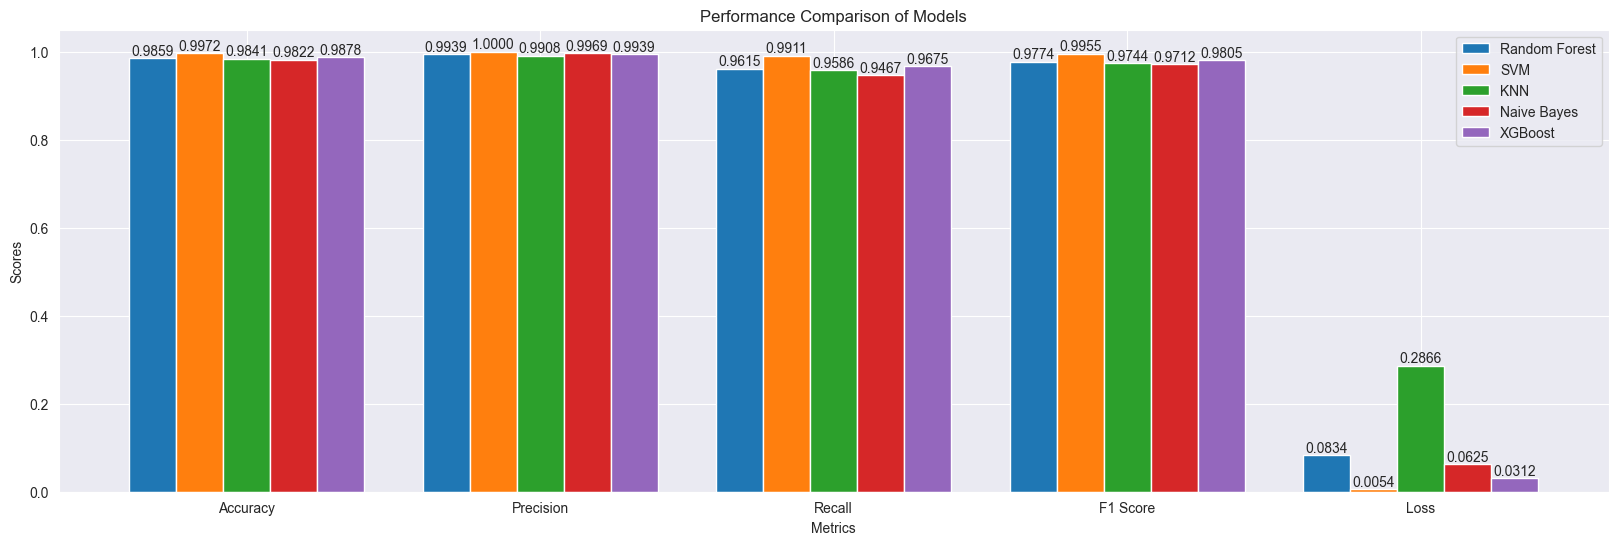
\includegraphics[width=\linewidth]{images/models_performance_train}
    \caption{Comparison of Models' Performance on Training Dataset}
    \label{fig:models_performance_train}
\end{figure}

\begin{itemize}
    \item \textbf{Accuracy:}
    \begin{itemize}
        \item SVM exhibits the highest accuracy (0.9972).
        \item KNN (0.9841), Random Forest (0.9859), Naive Bayes (0.9822), and XGBoost (0.9878) show very competitive and high accuracy scores, all above 0.98.
    \end{itemize}

    \item \textbf{Precision:}
    \begin{itemize}
        \item SVM achieves perfect precision (1.0000).
        \item Random Forest (0.9939), KNN (0.9908), Naive Bayes (0.9969), and XGBoost (0.9939) also demonstrate exceptionally high precision, all above 0.99.
    \end{itemize}

    \item \textbf{Recall:}
    \begin{itemize}
        \item SVM shows the highest recall (0.9911).
        \item XGBoost (0.9675) and Random Forest (0.9615) follow with high recall scores.
        \item KNN (0.9586) and Naive Bayes (0.9467) have slightly lower recall compared to the others, but still maintain strong performance.
    \end{itemize}

    \item \textbf{F1 Score:}
    \begin{itemize}
        \item SVM leads with the highest F1 Score (0.9955).
        \item XGBoost (0.9805) and Random Forest (0.9774) also have excellent F1 Scores, indicating a good balance between precision and recall.
        \item KNN (0.9744) and Naive Bayes (0.9712) show robust F1 Scores as well.
    \end{itemize}

    \item \textbf{Loss:}
    \begin{itemize}
        \item SVM has the lowest loss value (0.0054), indicating the best model fit according to this metric.
        \item XGBoost (0.0312) and Random Forest (0.0834) also have relatively low loss values.
        \item Naive Bayes (0.0625) has a moderate loss.
        \item KNN exhibits the highest loss among the models (0.2866).
    \end{itemize}

    \item \textbf{Overall Observations from the Chart:}
    \begin{itemize}
        \item Across the metrics of Accuracy, Precision, Recall, and F1 Score, SVM consistently performs as the top model or among the top performers.
        \item All models demonstrate very high performance (scores generally $>$ 0.94) for Accuracy, Precision, Recall, and F1 Score, suggesting the effectiveness of the underlying task.
        \item In terms of Loss (where lower is better), SVM is distinctly superior, followed by XGBoost.
        KNN shows a significantly higher loss compared to the other models.
    \end{itemize}
\end{itemize}

\begin{table}[H]
    \centering
    \caption{Model Performance Comparison (Based on Bar Chart)}
    \setlength{\tabcolsep}{3pt}
    \renewcommand{\arraystretch}{1.2}
    \resizebox{240pt}{!}{
        \begin{tabular}{|p{2.8cm}|p{2.8cm}|}
            \hline
            \textbf{Model} & \textbf{Key Analysis}                                                                      \\
            \hline
            Random Forest  & High overall performance. Excellent precision, strong recall \& F1. Moderate loss.         \\
            \hline
            SVM            & Top performer across all metrics. Perfect precision, highest Acc, Recall, F1. Lowest loss. \\
            \hline
            KNN            & Strong performance, slightly below RF / XGBoost. Highest loss among models.                \\
            \hline
            Naive Bayes    & Very high precision. Recall is the lowest among models, impacting F1 slightly. Low loss.   \\
            \hline
            XGBoost        & Excellent performance, second to SVM overall. Very low loss. Strong recall \& F1.          \\
            \hline
        \end{tabular}
    }
    \label{tab:model_performance_barchart}
\end{table}

\subsection{On the Validating Dataset}
\label{subsec:on-the-validating-dataset}
\begin{figure}[H]
    \centering
    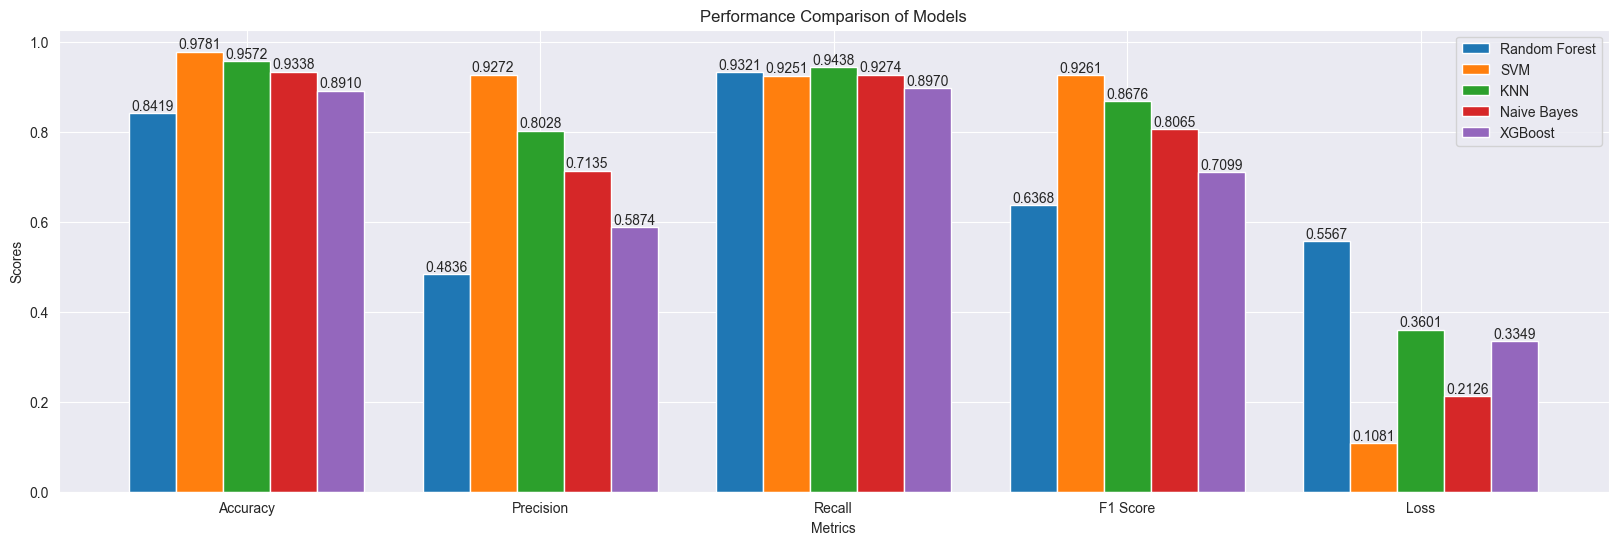
\includegraphics[width=\linewidth]{images/models_performance_validating}
    \caption{Comparison of Models' Performance on Validating Dataset}
    \label{fig:models_performance_validating}
\end{figure}

\begin{itemize}
    \item \textbf{General Trend Compared to Previous Data:}
    \begin{itemize}
        \item A significant drop in performance is observed across all models and most metrics (Accuracy, Precision, F1 Score) when comparing to the previously analyzed dataset (which had near-perfect scores). Recall scores are somewhat more varied, with some models maintaining high recall. Loss values have generally increased.
        \item This substantial decrease strongly suggests that the models may have overfit to the previous dataset, or that this new dataset presents a more challenging distribution, is inherently more complex, or has a different class balance. The previous high scores might not have been indicative of true generalization capability.
    \end{itemize}

    \item \textbf{Accuracy:}
    \begin{itemize}
        \item SVM exhibits the highest accuracy (0.9781) on this dataset, maintaining strong performance, though lower than its previously observed near-perfect score.
        \item KNN follows with a good accuracy of 0.9572.
        \item Naive Bayes (0.9338), XGBoost (0.8910), and Random Forest (0.8419) show a more considerable drop in accuracy. Random Forest's accuracy is now the lowest.
    \end{itemize}

    \item \textbf{Precision:}
    \begin{itemize}
        \item SVM leads with the highest precision (0.9272), a significant decrease from its previous perfect score but still the best.
        \item KNN (0.8028) and Naive Bayes (0.7135) maintain moderate precision.
        \item Random Forest (0.4836) and XGBoost (0.5874) show a very sharp decline in precision, indicating a large increase in false positives on this new dataset. This is a major change from their previously high precision.
    \end{itemize}

    \item \textbf{Recall:}
    \begin{itemize}
        \item KNN achieves the highest recall (0.9438) on this dataset.
        \item Random Forest (0.9321), SVM (0.9251), and Naive Bayes (0.9274) also maintain high recall scores, suggesting they are still effective at identifying positive instances.
        \item XGBoost's recall (0.8970) is also high, though slightly lower than the others in this group.
        \item The high recall for models like RF and KNN, despite lower precision, suggests they are casting a wide net, correctly identifying positives but also incorrectly flagging many negatives.
    \end{itemize}

    \item \textbf{F1 Score:}
    \begin{itemize}
        \item SVM has the highest F1 Score (0.9261), indicating the best balance between its high precision and high recall on this dataset.
        \item KNN (0.8676) also shows a good F1 Score.
        \item Naive Bayes (0.8065), XGBoost (0.7099), and Random Forest (0.6368) have lower F1 Scores, primarily impacted by their significant drop in precision (for RF and XGBoost) or a less optimal balance.
    \end{itemize}

    \item \textbf{Loss:}
    \begin{itemize}
        \item SVM maintains the lowest loss (0.1081), consistent with its strong performance across other metrics, though this loss is much higher than its previous near-zero loss.
        \item Naive Bayes (0.2126) has the next lowest loss.
        \item XGBoost (0.3349) and KNN (0.3601) have moderate loss values.
        \item Random Forest exhibits the highest loss (0.5567) on this dataset, correlating with its lower precision and accuracy.
    \end{itemize}

    \item \textbf{Overall Observations and Key Changes from Previous Dataset:}
    \begin{itemize}
        \item SVM demonstrates the most robust generalization, leading in Accuracy, Precision, F1 Score, and having the lowest Loss on this new, more challenging dataset. While its scores have decreased from the (assumed) training set, the drop is less severe compared to some other models.
        \item Random Forest and XGBoost show a dramatic decrease in Precision, leading to significantly lower F1 Scores. This suggests they might be particularly sensitive to changes in data distribution or may have learned overly specific patterns from the previous dataset. Their high recall now comes at the cost of many false positives.
        \item KNN, while having the highest loss previously, now shows a more competitive F1 score due to maintaining high recall and moderate precision. Its loss is still relatively high but not the outlier it was.
        \item Naive Bayes maintains relatively stable performance, with its precision dropping but recall remaining high.
        \item The major changes in performance indicate that this new dataset likely differs significantly from the one previously evaluated (assumed to be training/easier validation). This could be due to different underlying data characteristics, a shift in the data distribution (concept drift), or the presence of more noise or outliers. The previous near-perfect scores for some models were likely not representative of real-world generalization.
    \end{itemize}
\end{itemize}

\begin{table}[H]
    \centering
    \caption{Model Performance Comparison (Based on Validating Dataset)}
    \setlength{\tabcolsep}{3pt}
    \renewcommand{\arraystretch}{1.2}
    \resizebox{240pt}{!}{
        \begin{tabular}{|p{2.8cm}|p{2.8cm}|}
            \hline
            \textbf{Model} & \textbf{Key Analysis}                                                                           \\
            \hline
            Random Forest  & Lowest Acc. Very low Prec., high Recall (many FPs). Highest Loss. Significant performance drop. \\
            \hline
            SVM            & Best performer overall. Highest Acc, Prec, F1. Lowest Loss. Most robust generalization.         \\
            \hline
            KNN            & Good Acc. Highest Recall. Moderate Prec \& F1. High Loss. Performance drop but recall strong.   \\
            \hline
            Naive Bayes    & Moderate Acc                            \& Prec. High Recall. Second lowest Loss. Performance drop but relatively stable.   \\
            \hline
            XGBoost        & Moderate Acc. Low Prec., high Recall (many FPs). Moderate Loss. Significant drop in Prec/F1.    \\
            \hline
        \end{tabular}
    }
    \label{tab:model_performance_new_barchart}
\end{table}


    \section{Contribution}
    \label{sec:contribution}

    The following table represents the contribution of each member, note that whichever member handles whichever task will also write the report for that task.

    \begin{table}[h]
        \centering
        \caption{Members Contributions}
        \setlength{\tabcolsep}{2pt} % Reduce column spacing
        \renewcommand{\arraystretch}{1} % Adjust row spacing
        \resizebox{240}{!}{ % Fit within column width
            \begin{tabular}{|l|c|c|c|}
                \hline
                \textbf{ID} & \textbf{Member}        & \textbf{Contribution}                         & \textbf{Progress} \\
                \hline
                522H0036    & Luong Canh Phong       & Overseer, Implementation and Handling Report  & 100\%             \\
                520H0341    & Nguyen Thai Bao        & Research and Evaluating Models                & 100\%             \\
                522H0030    & Le Tan Huy             & Preprocessing the Dataset                     & 100\%             \\
                522H0008    & Dao Minh Phuc          & Visualizing the Dataset                       & 100\%             \\
                522H0136    & Nguyen Nhat Phuong Anh & Research Business and Visualizing the Dataset & 100\%             \\
                \hline
            \end{tabular}
        }
        \label{tab:contributions}
    \end{table}


    \section{Conclusion}
    \label{sec:conclusion}
    This paper addressed spam email detection through data preprocessing and the application of several machine learning models.
    Initial NLP-driven data exploration identified key email characteristics like headers, HTML elements, and spam-related terms, alongside a right-skewed email length distribution, underscoring the need for the implemented robust preprocessing pipeline.
    Five models—Random Forest, SVM, KNN, Naive Bayes, and XGBoost—were evaluated.

    While all models performed exceptionally well on the training data, with SVM achieving near-perfect scores, the validation dataset provided a clearer picture of generalization.
    SVM consistently emerged as the most robust model, leading in accuracy (0.9781), precision (0.9272), F1-score (0.9261), and achieving the lowest loss.
    In contrast, other models, particularly Random Forest and XGBoost, experienced significant drops in precision and overall performance, indicating potential overfitting or sensitivity to data variations.
    KNN maintained high recall but at the cost of precision, while Naive Bayes showed more stable, albeit moderate, performance.

    The general performance decline from training to validation highlights the critical challenge of overfitting and the necessity of evaluating models on unseen data.
    SVM's superior generalization capabilities make it a strong candidate for spam classification.
    This comparative analysis provides valuable insights for model selection in similar tasks.
    Future directions could involve exploring advanced feature engineering or deep learning approaches.


    \begin{thebibliography}{00}
        \bibitem{b1}
        \textit{XGBoost Documentation — xgboost 3.0.1 documentation}.
        (n.d.). https://xgboost.readthedocs.io/

        \bibitem{b2}
        \textit{scikit-learn: machine learning in Python — scikit-learn 0.16.1 documentation}.
        (n.d.). https://scikit-learn.org/

        \bibitem{b3}
        TensorFlow.
        (n.d.). \textit{TensorFlow}.
        https://www.tensorflow.org/

        \bibitem{b4}
        Wikipedia contributors.
        (2025, April 21). \textit{Cross-entropy}.
        Wikipedia.
        https://en.wikipedia.org/wiki/Cross\_entropy\#Cross-entropy\_loss\_function\_and\_logistic\_regression

        \bibitem{b5}
        Shannon, C. E., \& Weaver, W. (1949).
        A Mathematical Theory of Communication. \textit{Bell System Technical Journal}, \textit{27}(4), 623–656.
        https://doi.org/10.1002/j.1538-7305.1948.tb00917.x

        \bibitem{b6}
        Chen, T., \& Guestrin, C. (2016).
        XGBoost: a Scalable Tree Boosting System. \textit{Proceedings of the 22nd ACM SIGKDD International Conference on Knowledge Discovery and Data Mining - KDD ’16}, \textit{1}(1), 785–794.
        https://doi.org/10.1145/2939672.2939785

        \bibitem{b7}
        Breiman, L. (2001). \textit{Random Forests}.
        https://www.stat.berkeley.edu/~breiman/randomforest2001.pdf

        \bibitem{b8}
        Cortes, C., \& Vapnik, V. (1995).
        Support-vector networks. \textit{Machine Learning}, \textit{20}(3), 273–297.
        https://doi.org/10.1007/bf00994018

        \bibitem{b9}
        \textit{Pattern Recognition and Machine Learning (Information Science and Statistics): Bishop, Christopher M.: 9780387310732: Amazon.com: Books}.
        (n.d.). https://www.amazon.com/Pattern-Recognition-Machine-Learning-Information/dp/0387310738

        \bibitem{b10}
        \textit{Elements of Statistical Learning: data mining, inference, and prediction. 2nd Edition.} (n.d.).
        https://hastie.su.domains/ElemStatLearn/

        \bibitem{b11}
        \textit{Machine Learning: A Probabilistic Perspective (Adaptive Computation and Machine Learning series): Murphy, Kevin P.: 9780262018029: Amazon.com: Books}.
        (n.d.). https://www.amazon.com/Machine-Learning-Probabilistic-Perspective-Computation/dp/0262018020

        \bibitem{b12}
        \textit{Introduction to Machine Learning, fourth edition (Adaptive Computation and Machine Learning series): Alpaydin, Ethem: 9780262043793: Amazon.com: Books}.
        (n.d.). https://www.amazon.com/Introduction-Machine-Learning-Ethem-Alpaydin/dp/0262043793

        \bibitem{b13}
        \textit{Data Mining: Concepts and Techniques (The Morgan Kaufmann Series in Data Management Systems): Han, Jiawei, Kamber, Micheline, Pei, Jian: 9780123814791: Amazon.com: Books}.
        (n.d.). https://www.amazon.com/Data-Mining-Concepts-Techniques-Management/dp/0123814790

        \bibitem{b14}
        \textit{David MacKay: Information Theory, Inference, and Learning Algorithms: The book}.
        (n.d.). https://www.inference.org.uk/mackay/itila/book.html

        \bibitem{b15}
        \textit{Support vector Machines (Information Science and Statistics): Steinwart, Ingo, Christmann, Andreas: 9780387772417: Amazon.com: Books}.
        (n.d.). https://www.amazon.com/Support-Machines-Information-Science-Statistics/dp/0387772413

        \bibitem{b16}
        Godoy, D. (2025, March 7). \textit{Understanding binary cross-entropy / log loss: a visual explanation}.
        Towards Data Science.
        https://towardsdatascience.com/understanding-binary-cross-entropy-log-loss-a-visual-explanation-a3ac6025181a

        \bibitem{b17}
        Yıldırım, S. (2025, January 18). \textit{K-Nearest Neighbors (KNN) – explained}.
        Towards Data Science.
        https://towardsdatascience.com/k-nearest-neighbors-knn-explained\
%        \bibitem{b12} Tpoint Tech, ``Apriori Algorithm, ''\\\
%        [Online]. Available: \href{https://www.tpointtech.com/apriori-algorithm}{https://www.tpointtech.com/apriori-algorithm}
%        \bibitem{b6} Databricks, ``MapReduce, '' Databricks Glossary, 2025.\\\
%        [Online]. Available: \href{https://www.databricks.com/glossary/mapreduce}{https://www.databricks.com/glossary/mapreduce}
%        \bibitem{b1} J. S. Park and M. S. Chen, ``Using a hash table to eliminate candidates in a frequent itemset mining algorithm, '' \textit{IEEE Trans. Knowl. Data Eng.}, vol. 7, no. 3, pp. 464--472, 1995.
%        \bibitem{b2} J. Han, J. Pei, and Y. Yin, ``Mining frequent patterns without candidate generation, '' \textit{ACM SIGMOD Rec.}, vol. 29, no. 2, pp. 1--12, 2000.
%        \bibitem{b3} PySpark Documentation, ``PySpark API Documentation, '' 2025.\\\
%        [Online]. Available: \url{https://spark.apache.org/docs/latest/api/python}
%        \bibitem{b4} PySpark Documentation, ``pyspark.ml.feature.MinHashLSH, '' Apache Spark, 2025.\\\
%        [Online]. Available: \href{https://spark.apache.org/docs/latest/api/python/reference/api/pyspark.ml.feature.MinHashLSH}{https://spark.apache.org/docs/latest/api/python/refer\-ence/api/pyspark.ml.feature.MinHashLSH}
%        \bibitem{b5} Amazon Web Services, ``Jaccard similarity, '' AWS Neptune Analytics Documentation, 2024.\\\
%        [Online]. Available: \href{https://docs.aws.amazon.com/neptune-analytics/latest/userguide/jaccard-similarity.html}{https://docs.aws.amazon.com/neptune-analytics/latest/userguide/jaccard-similarity.html}
    \end{thebibliography}

    \medskip
    Link to Demo:
    https://truedevil666-anti-spam-mail.hf.space/?logs=container\&\_\_theme=system
\end{document}